\chapter{Machine Learning Basics II}
\section{Linear Regression}
Notation
\begin{itemize}
    \item m = Number of training examples
    \item x's = "input" variables/features
    \item y's = "output" variable/target variable
    \item $\{(x^{(i)},y^{(i)})\}$ = Training set
    \begin{flushleft}
        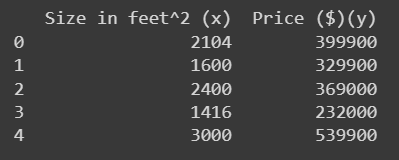
\includegraphics[scale = 0.7]{images/Training set.png}
    \end{flushleft}
    \item $h_{\theta}(x)$ = Hypothesis
\end{itemize}
Given a function $h_{\theta}(x)$ (e.g. $h_{\theta}(x) = \theta_{0} + \theta_{1}x$), choose $\theta_{0} \theta_{1}$ so that $h_{\theta}(x)$ is closed to $y$ in our training set $\{(x^{(i)},y^{(i)})\}$.
\begin{center}
    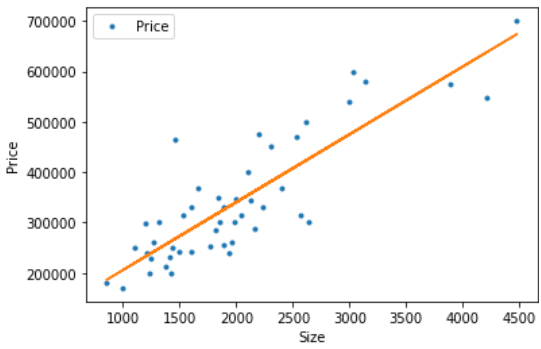
\includegraphics{images/Linear Ref.png}
\end{center}
To do that, we need to define a measure of the committed error, a \textbf{cost function} $J(\theta_{0},\theta_{1})$.
The goal is to find $\theta_{0} \theta_{1}$ in order to minimize $J(\theta_{0},\theta_{1})$ (e.g sum of square distances).
\[minimize_{\theta_{0} \theta_{1}}\frac{1}{2m}\sum_{i = 1}^{m}(h_{\theta}(x^{(i)}) - y^{(i)})^{2}\]

\subsection{Example with only one parameter}
Let's consider a simple example of linear regression with a function $h_{\theta}(x) = \theta_{1}x$ and a cost function $J(\theta_{1}) = \frac{1}{2m}\sum_{i = 1}^{m}(h_{\theta}(x^{(i)}) - y^{(i)})^{2}$.
\begin{center}
    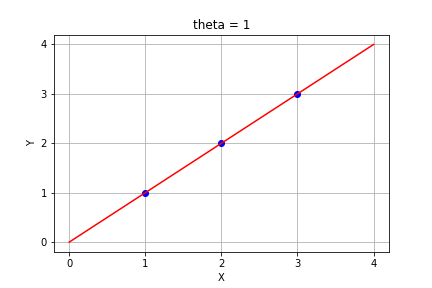
\includegraphics[scale = 0.7]{images/Simple liner reg.png}
\end{center}
As you can see from the graph above, our training set is composed by 3 points $\{(1,1), (2,2), (3,3)\}$. In this simple example the function $h_{\theta}(x)$ that perfectly fits the training set is the one with the parameter $\theta_{1} = 1$. In fact, if we compute the cost function $J(\theta_{1})$ with respect to $\theta_{1} = 1$, the result is 0 (minimized).
\[J(\theta_{1}) = \frac{1}{2m}\sum_{i = 1}^{m}(h_{\theta}(x^{(i)}) - y^{(i)})^{2}\]
\[= \frac{1}{2m}\sum_{i = 1}^{m}(\theta_{1}x^{(i)} - y^{(i)})^{2}\]
\[= \frac{1}{2m}(0+0+0)^2 = 0\]
But let's see what happens for different values of $\theta_{1}$.
\begin{itemize}
    \item $\theta_{1} = \frac{1}{2}$ $J(\theta_{1}) \approx 0.67$
    \item $\theta_{1} = 0$ $J(\theta_{1}) \approx 2.33$
    \item $\theta_{1} = -\frac{1}{2}$ $J(\theta_{1}) \approx 5.25$
\end{itemize}
\begin{center}
    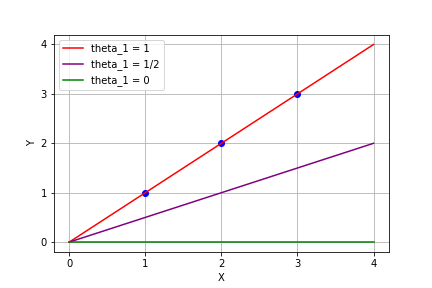
\includegraphics[scale = 0.7]{images/Simple liner reg (colors).png}
\end{center}
Now we can plot the values of $\theta_{1}$ on the \textbf{X} axis and the values of $J(\theta_{1})$ on the \textbf{Y} axis. The shape of $J(\theta_{1})$ will be the following:
\begin{figure}[h]
    \centering
    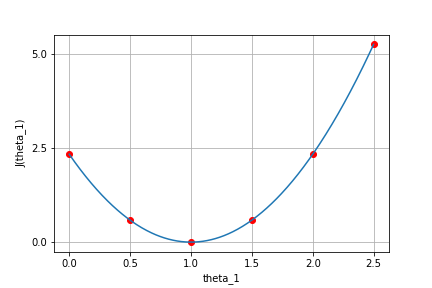
\includegraphics[scale = 0.7]{images/J.png}
    \label{Fig 1}
    \caption{Cost function J}
\end{figure}\newline
We obtain this \textbf{convex} function that has its minimum, for these specific $h_{\theta_{1}}(x^{(i)})$ and $y^{i}$, in 0. This principle is also valid for $n$-dimensional functions but the graphic representation is not that easy.\newline
How can we find $\theta_{1}$ in an automatic way?
\subsection{Gradient descent}
\textbf{Derivative:}\newline
The derivative tells us the slope of a function at any point. Given a point:
\begin{itemize}
    \item Positive derivative means that the function increases at that point
    \item Negative derivative means that the function decreases at that point.
    \item Null derivative means that there is a stationary point (minimum, maximum or saddle point).
\end{itemize}
Starting from a random configuration of $\theta$, each parameter is updated in the following way:
\[\theta_{k+1} = \theta_{k} - \eta \nabla J(\theta_{k})\]
where: 
\begin{itemize}
    \item $\nabla J(\theta_{k})$ is the partial derivative of the cost function in $\theta_{k}$.
    \item $\theta = \{\theta_{0},...,\theta_{n}\}$
    \item The parameter $\eta > 0$ is known as the \textit{learning rate}. 
\end{itemize}
Let's consider again the previous example with hypothesis function $h_{\theta}(x) = \theta_{1}x$. Our goal is to apply gradient descent algorithm in order to find a value of $\theta_{1}$ in which the partial derivative of $J$ is 0 where the function has a local minimum (so the cost function is minimized). For our simple example that point is $\theta_{1} = 1$\newline
Given the expression: 
\[\theta_{1} := \theta_{1} - \eta \frac{\partial}{\partial \theta_{1}}J(\theta_{1})\]
The derivative term $\frac{\partial}{\partial \theta_{1}}J(\theta_{1})$ can be:
\begin{itemize}
    \item $\geq 0$ it means that the function is increasing, so we are decreasing $\theta_{1}$ in the \textit{right direction}.
    \item $\leq 0$ it means that the function is decreasing, so we are increasing $\theta_{1}$ in the \textit{right direction}
\end{itemize}
\begin{flushleft}
    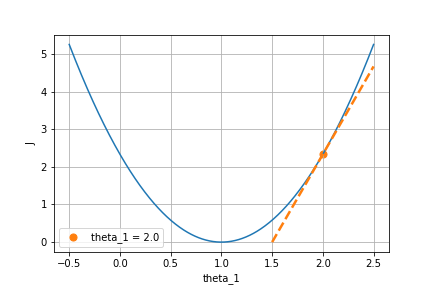
\includegraphics[scale=0.5]{images/partial derivative.png}
    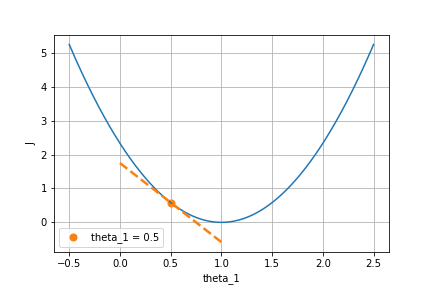
\includegraphics[scale=0.5]{images/partial derivative_1.png}
\end{flushleft}
\begin{center}
    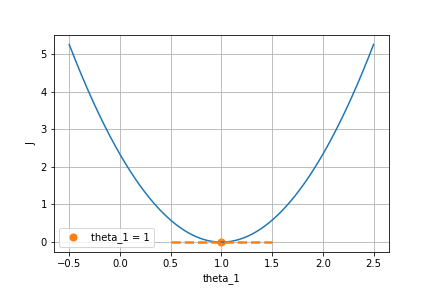
\includegraphics[scale=0.5]{images/partial derivative_2.png}
\end{center}
if $\eta$ is too small, gradient descent can be slow. Anyway, if it is too large, it can overshoot the minimum (fail to converge).\newline
The partial derivative of the cost function used in the previous example is the following:
\[\frac{\partial}{\partial \theta_{1}} \frac{1}{2m}\sum_{i=1}^{m}(\theta_{1}x^{(i)} - y^{(i)})^{2}\]
\[= \frac{1}{m}\sum_{i=1}^{m}(\theta_{1}x^{(i)} - y^{(i)})x^{(i)}\]
The algorithm also works with an n-dimensional input (multiple parameters $\theta$).
There are different ways in which the algorithm can be applied:
\begin{itemize}
    \item \textbf{Batch gradient descent:} Each step of gradient descent uses all training examples.
    \item \textbf{Stochastic gradient descent:} Update the parameters for each training case in turn, according to its own gradients.
    \item \textbf{Mini-batch gradient descent}: Update the parameters using a subset of the sample.
\end{itemize}
\subsection{Binary Classification}
\textbf{Classification: } determine to which discrete category a specific example belongs to
\begin{itemize}
    \item Binary classification: Two possible labels
    \item Multi-class classification: multiple possible labels
\end{itemize}
We can perform binary classification using the Linear Regression technique seen before. What we have to do is to choose a \textit{Decision rule}.
Let's assume that we have two labels for our classes $Y \equiv \{(-1,+1)\}$. The decision rule could be $y = sign(h_{\theta}(x))$:
\begin{itemize}
    \item if $h_{\theta}(x) \geq 0$, predict $y=1$
    \item if $h_{\theta}(x) < 0$, predict $y=-1$
\end{itemize}
If we have $Y \equiv \{(0,+1)\}$ the decision rule could be instead:
\begin{itemize}
    \item if $h_{\theta}(x) \geq 0.5$, predict $y=1$
    \item if $h_{\theta}(x) < 0.5$, predict $y=0$
\end{itemize}
This specifies a \textit{linear classifier}. It has a linear boundary (hyperplane) which separates the space.
\begin{center}
    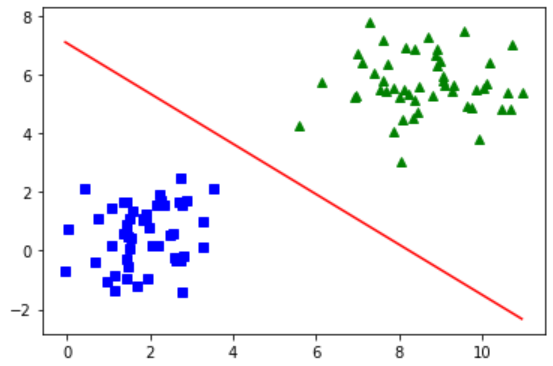
\includegraphics[scale = 0.7]{images/Hyperplanes in R^2.png}
\end{center}
In 2D it is a line, in 3D is a plane and so on.\newline
Applying linear regression to classification tasks is not always a great idea since it is very influenced by outliers.
\section{Logistic Regression}
Although the term regression appears in its name, logistic regression is a classification algorithm.
The hypothesis space is composed by functions of type:
\[h_{\theta}(x) = g(\theta^{T},x) = \frac{1}{1 + e^{-\theta^{T}x}}\]
where $g(z) = \frac{1}{1 + e^{-z}}$ is the sigmoid/logistic function.\newline
\textbf{Example:} $h_{\theta}(x) = \frac{1}{1 + e^{-(\theta_{0} + \theta_{1}x)}}$
\begin{figure}[h]
    \centering    
    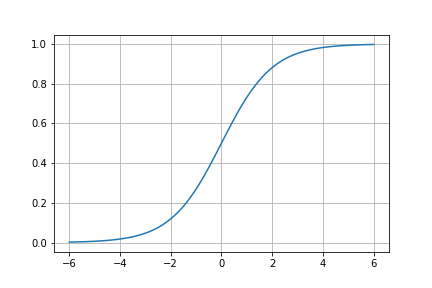
\includegraphics[scale=0.5]{images/sigmoid.png}
    \caption{$\theta_{0} = 0$, $\theta_{1} = 1$}
    \label{fig:sigmoid}
\end{figure}
\begin{figure}[h]
    \centering
    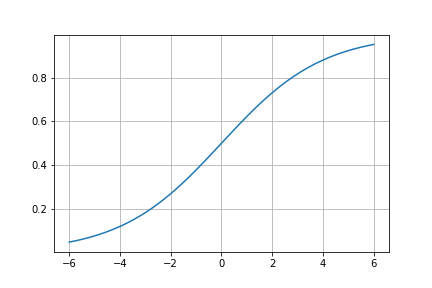
\includegraphics[scale=0.5]{images/sigmoid_1.png}
    \caption{$\theta_{0} = 0$, $\theta_{1} = 1$}
    \label{fig:sigmoid_1}
\end{figure} \newline
Note that $\theta_{0}$ and $\theta_{1}$ determine the shape of the function.\newline
As in the case of Linear regression, we have to choose a \textit{Decision rule}. Suppose to predict: 
\begin{itemize}
    \item $y = 1$ if $h_{\theta}(x) \geq 0.5$
    \item $y = 0$ if $h_{\theta}(x) < 0.5$ 
\end{itemize}
So, although the sigmoid function is a non-linear function, Logistic regression is still a linear model because the \textbf{decision boundary} is linear. One of the advantages of using Logistic regression is that is more robust with respect to \textit{outliers}
\begin{center}
    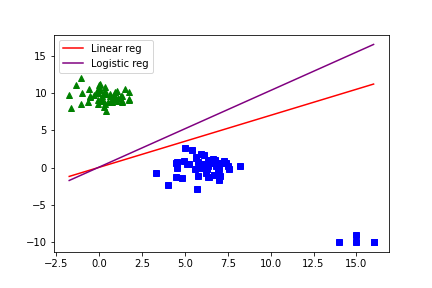
\includegraphics[scale=0.7]{images/linear vs log.png}
\end{center}
Finally, The cost function defined for logistic regression is not Mean Square Error. This is because it is no more a \textbf{convex} function when $h_{\theta}(x) = \frac{1}{1 + e^{-\theta^{T}x}}$. So, in order to optimize gradient descent algorithm, we will use \textbf{Cross-Entropy Cost Function}: $J(\theta) = \frac{1}{m} \sum_{i = 1}^{m}cost(h_{\theta}(x^{(i)}), y^{(i)})$ \newline
where $cost(h_{\theta}(x^{(i)}), y^{(i)})$ = 
\[
    \begin{cases}
         - \log(h_{\theta}(x^{(i)}))  & y^{(i)} = 1\\
         - \log(1 - h_{\theta}(x^{(i)})) & y^{(i)} = 0
    \end{cases}
\]
Simplified notation:
\[J(\theta) = - \frac{1}{m}\sum_{i=1}^{m}( y^{(i)} \cdot \log(h_{\theta}(x^{(i)})) + (1 - y^{(i)}) \cdot \log(1 - h_{\theta}(x^{(i)}))  )\]
This is a \textbf{convex} function, so we can use the gradient descent update rule mentioned before \footnote{Note that even with Mean Square error cost function we could have used gradient descent algorithm, but the derivative of $J(\theta)$ would have been different}:
\[\theta_{j} := \theta_{j} - \eta \frac{\partial}{\partial \theta_{j}}J(\theta) = \theta_{j} - \frac{\eta}{m}\sum_{i=1}^{m}(h_{\theta}(x^{(i)}) - y^{(i)})x_{j}\]

